\title{Measurement: The Simple Pendulum}
\author{An Introduction to Physics through Experiments}
\date{}

\maketitle

\section{Objectives}

\begin{enumerate}
    \item Understanding data collection
    \item Understanding data representation
    \item Understanding data interpretation
    \item To observe the variation of the time period of a simple pendulum with different parameters.
\end{enumerate}

\section{Introduction}

In this preliminary experiment you will be exposed to the ideas of measurement, data collection, and elementary data interpretation using the simple pendulum. 

\subsection{Data Collection}

\subsubsection{Tables}

In this laboratory you will be observing physical phenomena that are relatively well understood. In general, you will be asked to either verify certain formulae or to extract the value of certain physical quantities from them. As a result, you would usually have an \textbf{independent variable} that you will change over the course of collecting data, and a \textbf{dependent variable} which you will \textit{measure}. The data that you will take will have to be taken systematically, in order for you to make full use of it. As a result, it is imperative that you learn to tabulate your raw data well, so that you do not run into trouble later.

You will need a lab (auxiliary) notebook within which you will take your readings. It is essential that none of these readings be changed; if you have noted down something wrong, strike it out, and write down the correct value. However, it is essential to have a record of all the data you have taken. Remember: this does not need to be neat, only understandable to \textbf{you}. The TA or course instructor will have to initial your data. Do not underestimate the temptation to change your data: never discount points unless you have adequate reason to do so, and \textbf{never} change the value of a reading so that it fits a trend that you imagine is the `right' one.


There is no strict `right' way to tabulate data. Here is a simple example: 

\begin{table}[!htb]
\centering
\begin{tabular}{|C{4cm}|C{2cm}|C{2cm}|C{2cm}|C{4cm}|}
\hline
\rowcolor{Gray}
\textbf{Independent Variable {\color{gray}(unit)}} & \multicolumn{3}{|c|}{\textbf{Dependent Variable {\color{gray}(unit)}}} &\textbf{Derived Quantity {\color{gray}(unit)}} \\ \hline
{} & Trial 1 & Trial 2 & Trial 3 & {} \\
\hline
{} & {} & {} & {} & {} \\
\hline
{} & {} & {} & {} & {} \\
\hline
{} & {} & {} & {} & {} \\
 \hline
\end{tabular}
\caption{Sample data table}
\label{sampledata}
\end{table}

Spend some time deciding what data table to draw before beginning your experiment: it will help you decide what data to take.

\subsubsection{``How many readings should I take?''}

This is the question we hear the most often. The answer is of course that \textbf{it depends}. It certainly depends on the experimental setup, and it depends on the different types of uncertainties present in each measurement.

Ideally we imagine that any physical quantity that we are measuring has a `true' value, and some spread around this value.

One way to increase your confidence in experimental data is to repeat the same measurement many times. For example, one way to estimate the amount of time it takes something to happen is to simply time it once with a stopwatch. You can decrease the uncertainty in this estimate by making this same measurement multiple times and taking the average. The more measurements you take (provided there is no problem with the clock!), the better your estimate will be.

\subsection{Theory: The Simple Pendulum}

The simple pendulum is a point mass suspended from a string of negligible mass attached to a pivot point, as shown in Figure (\ref{simple}). 

\begin{figure}[!htb]
    \centering
    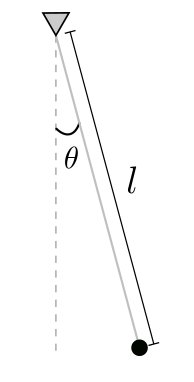
\includegraphics[scale=0.5]{figs/simplependulum.png}
    \caption{The Simple Pendulum}
    \label{simple}
\end{figure}

If a pendulum is set in motion so that is swings back and forth, its motion will be periodic. The time that it takes to make one complete oscillation is defined as the \textbf{time period} $T$ of the pendulum. Most of you will probably recognise the following formula for $T$: 

\begin{equation}
    T = 2 \pi \sqrt{\frac{l}{g}} 
    \label{TimeP}
\end{equation}

where $l$ is the length of the pendulum from its fixed point, and $g$ is the acceleration due to gravity. Not so many of you, however, will realise that this is only true for \textbf{small displacements} around the equilibrium position. In general, when the pendulum is displaced from its equilibrium position, it experiences a restoring force $m g \sin\theta$. The differential equation describing its motion can be obtained from Newton's Second Law  $m\vb{a} = \vb{F}$.

\begin{equation}
    m l \dv[2]{\theta}{t} = - m g \sin\theta
\end{equation}

This is a difficult differential equation to solve. In the approximation that the angle $\theta$ is very small, we can replace $\sin\theta \approx \theta$, and we are left with the following differential equation:

\begin{equation}
    \dv[2]{\theta}{t} + \frac{g}{l} \theta = 0
\end{equation}

It is in this approximation that the simple pendulum is a \textbf{simple harmonic oscillator}, a very important model that you will not stop seeing the end of. In general, a quantity $Q$ is considered observe simple harmonic variation with respect to some parameter $t$ (not necessarily time) if it satisfies the following differential equation:

\begin{equation*}
    \dv[2]{Q}{t} + \omega_0^2 Q = 0
\end{equation*}

where $\omega_0$ is the time period of the oscillation, and is related to the time period of the oscillation through 

\begin{equation*}
    T = \frac{2\pi}{\omega_0}
\end{equation*}

Comparing, you should see that in our case, $$\omega_0 = \sqrt{\frac{g}{l}}$$ and $$T = 2\pi \sqrt{\frac{l}{g}}$$

Thus, it should be clear that it is only when the amplitude is \textbf{small} that the time period follows this equation, since it is only then when you can approximate $\sin\theta$ with $\theta$.

In this introductory experiment you will begin by verifying the above formula for the time period for small angles. You will then attempt to explore any variation of the time period with angle.

\section{Apparatus}

\begin{enumerate}
    \item Metallic bobs of different materials
    \item A length of string
    \item A cork with a slit
    \item A retort stand with attached protractor
\end{enumerate}

\section{Suggested Procedure}

\paragraph{Question:} Which are the different physical quantities in this problem that can be varied to potentially change the time period\footnote{\textbf{Warning!} Do not use Equation (\ref{TimeP}) to answer this: we've already seen that that only works under certain special cases}?

\subsection{Part 1}

In this part of the experiment you will design a simple experiment to determine the variation of the time period with the mass of the bob.

\begin{enumerate}
    \item Begin by deciding which variables you need to fix, and which variables you will change.
    
    \item Draw out an appropriate table in your auxiliary notebooks. Mark out any important details that would help you remember what you've done when you re-read this. Remember to state not only what you have changed, but also what you have kept \textit{fixed}.
    
    \item Decide on the \textbf{number} of readings you will take. When you have arrived at a number, try to \textit{justify} it.
    
    \item Perform the necessary experiment, varying the relevant parameter. Note down your data.
    
    \item Plot an appropriate graph that accurately depicts your results.
\end{enumerate}

\paragraph{Question:} What is your conclusion? How confident are you of this conclusion?


\subsection{Part 2}

In this part of the experiment you will design a simple experiment to determine the variation of the time period with the length of the string from the pivot to the center of mass of the bob.

\begin{enumerate}
    \item Begin by deciding which variables you need to fix, and which variables you will change.
    
    \item Draw out an appropriate table in your auxiliary notebooks. Mark out any important details that would help you remember what you've done when you re-read this. Remember to state not only what you have changed, but also what you have kept \textit{fixed}.
    
    \item Decide on the \textbf{number} of readings you will take. When you have arrived at a number, try to \textit{justify} it.
    
    \item Perform the necessary experiment, varying the relevant parameter. Note down your data.
    
    \item Plot an appropriate graph that accurately depicts your results.
\end{enumerate}

\subsection{Part 3}

In this part of the experiment you will design a simple experiment to determine the variation of the time period with the angle of release of the bob.

\begin{enumerate}
    \item Begin by deciding which variables you need to fix, and which variables you will change.
    
    \item Draw out an appropriate table in your auxiliary notebooks. Mark out any important details that would help you remember what you've done when you re-read this. Remember to state not only what you have changed, but also what you have kept \textit{fixed}.
    
    \item Decide on the \textbf{number} of readings you will take. When you have arrived at a number, try to \textit{justify} it.
    
    \item Perform the necessary experiment, varying the relevant parameter. Note down your data.
    
    \item Plot an appropriate graph that accurately depicts your results.
\end{enumerate}


\paragraph{Note:} The repetition is -- of course -- intentional. We have found that students usually jump through these steps and -- as a result -- spend much of their time painstakingly collecting data that is of little or no use. It is essential that you spend some time deciding what exactly you want to collect, and how best you will represent it, before actually spending any time with the apparatus.



\section{Questions}

\paragraph{Question: } What would be the effect -- if any -- of changing the \textbf{shape} of the bob on the time period? Justify your answer.